\section{Đạo hàm}
\label{sec:derivative}

\subsection{Định nghĩa đạo hàm}

Trong Mục 2.1.1 của chương trước, chúng ta đã thấy rằng hai bài toán tưởng chừng không liên quan---bài toán tìm hệ số góc của tiếp tuyến và bài toán vận tốc tức thời---đều dẫn đến một khái niệm chung: giới hạn của tỉ số
$$
\dfrac{f(x) - f(a)}{x-a}
$$
khi $x$ tiến về $a$. Số thực này phản ánh tốc độ thay đổi của đại lượng $f(x)$ so với sự thay đổi của $x$.

Để củng cố ý tưởng này, chúng ta hãy xem xét lại bài toán tìm độ dốc của tiếp tuyến với đồ thị hàm số $f$ tại điểm $x_0$. Như trong Hình \ref{fig:tangent-slope}, ta có thể xấp xỉ tiếp tuyến bằng các cát tuyến $l_n$ đi qua hai điểm $(x_0, f(x_0))$ và $(x_0 + h_n, f(x_0 + h_n))$ trên đồ thị. Khi $h_n$ dần tiến về 0, các cát tuyến này sẽ tiến dần về tiếp tuyến của đồ thị tại điểm $(x_0, f(x_0))$.

Hệ số góc của cát tuyến $l_n$ được tính bởi công thức:
$$
\dfrac{f(x_0 + h_n) - f(x_0)}{(x_0 + h_n) - x_0} = \dfrac{f(x_0 + h_n) - f(x_0)}{h_n}
$$
Vì vậy, hệ số góc của tiếp tuyến chính là giới hạn của tỉ số này khi $h_n$ dần tiến về 0. Điều này dẫn chúng ta đến định nghĩa cốt lõi sau đây.

\begin{figure}[H]
	\centering
	\begin{tikzpicture}
		\begin{axis}[
			axis lines=middle,
			xmin=-1, xmax=8,
			ymin=-1, ymax=9,
			xtick={2, 3.5, 5, 6.5},
			xticklabels={$x_0$, $x_0+h_1$, $x_0+h_2$, $x_0+h_3$},
			ytick={2, 3, 4.5, 6.5},
			yticklabels={$f(x_0)$, $f(x_0+h_1)$, $f(x_0+h_2)$, $f(x_0+h_3)$},
			xlabel={},
			ylabel={},
			width=12cm,
			height=10cm,
			]
			% Define points
			\coordinate (P) at (axis cs:2,2);
			\coordinate (Q1) at (axis cs:3.5, 3);
			\coordinate (Q2) at (axis cs:5, 4.5);
			\coordinate (Q3) at (axis cs:6.5, 6.5);
			
			% % Draw secant lines
			% \addplot[domain=0:7.5, color=red, thick, samples=2, name path=l1] table {2 2 \\ 6.5 8.0625};
			% \addplot[domain=0:7.5, color=orange, thick, samples=2, name path=l2] table {2 2 \\ 5 5.5625};
			% \addplot[domain=0:7.5, color=brown, thick, samples=2, name path=l3] table {2 2 \\ 3.5 3.5625};
			
			% Draw the main function curve
			\addplot[domain=1:7, color=green!50!black, very thick, samples=100] {(1/9)*x^2 + (1/18)*x + 13/9} node[pos=0.9, right] {$f(x)$};
			
			% Draw points on the curve
			\fill (P) circle (1.5pt);
			\fill (Q1) circle (1.5pt);
			\fill (Q2) circle (1.5pt);
			\fill (Q3) circle (1.5pt);
			
			% Draw dashed lines for coordinates
			\draw[dashed] (axis cs:0, 2) -- (P);
			\draw[dashed] (axis cs:2, 0) -- (P);
			
			\draw[dashed] (axis cs:0, 3) -- (Q1);
			\draw[dashed] (axis cs:3.5, 0) -- (Q1);
			
			\draw[dashed] (axis cs:0, 4.5) -- (Q2);
			\draw[dashed] (axis cs:5, 0) -- (Q2);
			
			\draw[dashed] (axis cs:0, 6.5) -- (Q3);
			\draw[dashed] (axis cs:6.5, 0) -- (Q3);
			
			% Add labels for lines
			\node[above, color=red] at (axis cs:6, 8.5) {$l_1$};
			\node[above, color=orange] at (axis cs:5.5, 8.5) {$l_2$};
			\node[above, color=brown] at (axis cs:5, 8.5) {$l_3$};
			
		\end{axis}
	\end{tikzpicture}
	\caption{Bài toán hệ số góc của tiếp tuyến.}
	\label{fig:tangent-slope}
\end{figure}

\begin{definition}[Đạo hàm]
Cho hàm số $f$ xác định trên một khoảng mở chứa điểm $x_0$. \textbf{Đạo hàm} của $f$ tại $x_0$, ký hiệu là $f'(x_0)$, là số thực được định nghĩa bởi giới hạn:

\begin{importantbox}
    \[f'(x_0) = \limit{h}{0} \dfrac{f(x_0 + h) - f(x_0)}{h}\]
\end{importantbox}

nếu giới hạn này tồn tại. Khi đó, ta nói hàm $f$ \textbf{có đạo hàm} hay \textbf{khả vi} (differentiable) tại $x_0$.
\end{definition}

Ta cũng có thể viết lại định nghĩa đạo hàm bằng cách đặt $h = x - x_0$. Khi đó $h \to 0$ tương đương với $x \to x_0$, và ta có một dạng tương đương:

\begin{importantbox}
    \[f'(x_0) = \limit{x}{x_0} \dfrac{f(x) - f(x_0)}{x - x_0}\]
\end{importantbox}

% Nối tiếp nội dung của file chapters/03 - chapter3.tex

Một cách viết khác cũng rất phổ biến là sử dụng ký hiệu ``delta'' để biểu thị sự thay đổi. Nếu ta gọi $\Delta x = h$ là một số gia của biến $x$ tại $x_0$, thì lượng thay đổi tương ứng của giá trị hàm số $y=f(x)$ là $\Delta y = f(x_0 + \Delta x) - f(x_0)$. Khi đó, đạo hàm của $f$ tại $x_0$ chính là tỉ lệ thay đổi của $y$ so với $x$ khi $\Delta x$ vô cùng nhỏ:
$$
f'(x_0) = \limit{\Delta x}{0} \dfrac{f(x_0 + \Delta x) - f(x_0)}{\Delta x} = \limit{\Delta x}{0} \dfrac{\Delta y}{\Delta x}
$$

Vậy, đạo hàm của một hàm số tại một điểm đo lường \textbf{tốc độ thay đổi tức thời} của hàm số tại chính điểm đó. Khái niệm này là nền tảng của vô số ứng dụng trong khoa học và kỹ thuật, từ việc mô tả chuyển động của các vật thể trong vật lý đến việc tối ưu hóa lợi nhuận trong kinh tế.

Với định nghĩa chính xác về đạo hàm, giờ đây ta có thể định nghĩa một cách hình thức các khái niệm về tiếp tuyến và vận tốc đã được thảo luận trước đó.

\begin{itemize}
    \item \textbf{Tiếp tuyến:} Nếu hàm $f$ khả vi tại $x_0$, ta định nghĩa \textbf{tiếp tuyến} với đồ thị của hàm số $f$ tại điểm $P(x_0, f(x_0))$ là đường thẳng đi qua $P$ và có hệ số góc bằng $f'(x_0)$. Phương trình của tiếp tuyến này là:
    \begin{importantbox}
        \[y - f(x_0) = f'(x_0)(x - x_0)\]
    \end{importantbox}
    
    \item \textbf{Vận tốc tức thời:} Nếu $s(t)$ là hàm biểu thị vị trí của một vật trên một đường thẳng tại thời điểm $t$, và hàm $s$ khả vi tại $t_0$, thì \textbf{vận tốc tức thời} của vật tại thời điểm $t_0$ chính là $v(t_0) = s'(t_0)$.
\end{itemize}

\subsubsection{Các ví dụ tính đạo hàm bằng định nghĩa}

Bây giờ, chúng ta sẽ áp dụng định nghĩa để tính đạo hàm của một số hàm số cơ bản.

\begin{example}[Đạo hàm của hàm hằng]
Cho hàm số hằng $f(x) = c$ với mọi $x \in \R$. Hãy tìm đạo hàm của $f$.
\end{example}
\begin{solution}
Theo định nghĩa, tại một điểm $x_0$ bất kỳ:
$$
f'(x_0) = \limit{h}{0} \dfrac{f(x_0 + h) - f(x_0)}{h} = \limit{h}{0} \dfrac{c - c}{h} = \limit{h}{0} 0 = 0
$$
Vậy, $f'(x_0) = 0$ với mọi $x_0 \in \R$. Kết quả này hoàn toàn phù hợp với trực giác: một đại lượng không đổi thì có tốc độ thay đổi bằng 0.
\end{solution}

\begin{example}[Đạo hàm của hàm đồng nhất]
Tính đạo hàm của hàm số $f(x) = x$ tại một điểm $x_0$ bất kỳ.
\end{example}
\begin{solution}
Ta có:
$$
f'(x_0) = \limit{h}{0} \dfrac{f(x_0 + h) - f(x_0)}{h} = \limit{h}{0} \dfrac{(x_0 + h) - x_0}{h} = \limit{h}{0} \dfrac{h}{h} = \limit{h}{0} 1 = 1
$$
Vậy $f'(x_0) = 1$. Về mặt hình học, đồ thị của $y=x$ là một đường thẳng có hệ số góc bằng 1, nên tiếp tuyến tại mọi điểm trùng với chính nó và cũng có hệ số góc bằng 1.
\end{solution}

\begin{example}[Đạo hàm của hàm bậc hai]
Sử dụng định nghĩa, hãy tính đạo hàm của hàm số $f(x) = x^2$ tại điểm $x=x_0$.
\end{example}
\begin{solution}
Đầu tiên, ta tính số gia của hàm số:
$$
f(x_0 + h) - f(x_0) = (x_0 + h)^2 - x_0^2 = (x_0^2 + 2x_0h + h^2) - x_0^2 = 2x_0h + h^2
$$
Do đó, tỉ số của số gia là:
$$
\dfrac{f(x_0 + h) - f(x_0)}{h} = \dfrac{2x_0h + h^2}{h} = 2x_0 + h
$$
Lấy giới hạn khi $h \to 0$, ta được:
$$
f'(x_0) = \limit{h}{0} (2x_0 + h) = 2x_0
$$
Điều này có nghĩa là hàm $f(x) = x^2$ có đạo hàm tại mọi điểm $x_0$, và $f'(x_0) = 2x_0$.
\end{solution}

\begin{example}[Đạo hàm của hàm lũy thừa $f(x) = x^k$]
Với $k$ là một số nguyên dương, hãy tính đạo hàm của hàm $f(x) = x^k$ tại $x=x_0$.
\end{example}
\begin{solution}
Ta cần tính giới hạn của tỉ số $\dfrac{(x_0+h)^k - x_0^k}{h}$. Sử dụng công thức nhị thức Newton, ta có:
$$
(x_0+h)^k = x_0^k + kx_0^{k-1}h + \dfrac{k(k-1)}{2!}x_0^{k-2}h^2 + \dots + h^k
$$
Do đó:
\begin{align*}
\dfrac{(x_0+h)^k - x_0^k}{h} &= \dfrac{(x_0^k + kx_0^{k-1}h + \dots + h^k) - x_0^k}{h} \\
&= \dfrac{kx_0^{k-1}h + \dfrac{k(k-1)}{2!}x_0^{k-2}h^2 + \dots + h^k}{h} \\
&= kx_0^{k-1} + \dfrac{k(k-1)}{2!}x_0^{k-2}h + \dots + h^{k-1}
\end{align*}
Khi cho $h \to 0$, tất cả các số hạng chứa $h$ sẽ tiến về 0. Vì vậy:
$$
f'(x_0) = \limit{h}{0} \left( kx_0^{k-1} + \dfrac{k(k-1)}{2!}x_0^{k-2}h + \dots + h^{k-1} \right) = kx_0^{k-1}
$$
Vậy, $(x^k)' = kx^{k-1}$.
\end{solution}

\begin{example}[Đạo hàm của hàm căn thức]
Tính đạo hàm của hàm số $f(x) = \sqrt{x}$ (với $x > 0$).
\end{example}
\begin{solution}
Ta tính giới hạn bằng phương pháp nhân lượng liên hợp:
\begin{align*}
f'(x) = \limit{h}{0} \dfrac{\sqrt{x+h} - \sqrt{x}}{h} &= \limit{h}{0} \dfrac{(\sqrt{x+h} - \sqrt{x})(\sqrt{x+h} + \sqrt{x})}{h(\sqrt{x+h} + \sqrt{x})} \\
&= \limit{h}{0} \dfrac{(x+h) - x}{h(\sqrt{x+h} + \sqrt{x})} \\
&= \limit{h}{0} \dfrac{h}{h(\sqrt{x+h} + \sqrt{x})} \\
&= \limit{h}{0} \dfrac{1}{\sqrt{x+h} + \sqrt{x}} = \dfrac{1}{2\sqrt{x}}
\end{align*}
Giới hạn này tồn tại với mọi $x > 0$. Vậy, $(\sqrt{x})' = \dfrac{1}{2\sqrt{x}}$.
\end{solution}

\subsubsection{Đạo hàm như một hàm số}

Qua các ví dụ trên, ta thấy rằng để tìm công thức chung cho đạo hàm, việc định nghĩa đạo hàm như một hàm số mới sẽ tiện lợi hơn. Thay vì tính đạo hàm tại từng điểm $x_0$ riêng lẻ, ta định nghĩa \textbf{hàm đạo hàm} $f'$ có giá trị tại mỗi điểm $x$ là $f'(x)$.

\begin{tcolorbox}[colback=yellow!10!white, colframe=blue!75!black, fonttitle=\bfseries, boxrule=0.5pt, arc=2mm]
$$
f'(x) = \limit{h}{0} \dfrac{f(x+h) - f(x)}{h}
$$
\end{tcolorbox}

Cách tiếp cận này không chỉ giúp ta không cần giới thiệu thêm biến $x_0$ mà còn làm nổi bật vai trò của đạo hàm như một hàm số mới, được ``dẫn xuất'' từ hàm ban đầu.\footnote{Từ ``đạo hàm'' có thể có nghĩa sơ lược là đường hướng của hàm, có lẽ bắt nguồn từ thuật ngữ ban đầu mà Newton đưa ra là \textit{fluxion}. Ngày nay thuật ngữ đạo hàm trong tiếng Anh là \textit{derivative}, có nghĩa là dẫn xuất, từ một cái khác mà ra.}

Trong định nghĩa đạo hàm tại một điểm $x_0$, để thuận tiện ta yêu cầu điểm $x_0$ phải có một khoảng mở chứa nó nằm trong miền xác định của hàm. Mặc dù vậy, theo định nghĩa của giới hạn, để xét giới hạn trong định nghĩa đạo hàm thì giả thiết $x_0$ là một điểm tụ của miền xác định là đủ. Đôi khi yêu cầu ít hơn này được sử dụng, chẳng hạn nếu hàm xác định trên đoạn $[a, b]$ thì ta có thể định nghĩa \textbf{đạo hàm bên phải} tại $a$ (chỉ xét giới hạn bên phải) và \textbf{đạo hàm bên trái} tại $b$ (chỉ xét giới hạn bên trái).

\subsection{Liên hệ giữa khả vi và liên tục}

Một câu hỏi tự nhiên được đặt ra là: Mối liên hệ giữa một hàm số có đạo hàm và một hàm số liên tục là gì? Một cách trực quan, để một đồ thị có tiếp tuyến tại một điểm, nó không thể bị ``đứt'' hay có ``lỗ hổng'' tại điểm đó. Điều này gợi ý rằng tính khả vi là một điều kiện mạnh hơn tính liên tục.

Ta nói hàm số $f$ là \textbf{khả vi} (có vi phân) tại $x$ nếu $f$ có đạo hàm tại $x$. Ta có thể đoán rằng để $f$ khả vi tại $x$, tức là để tỉ số $\dfrac{f(x+h)-f(x)}{h}$ có giới hạn khi $h$ tiến về 0, thì tử số $f(x+h)-f(x)$ phải tiến về 0. Điều này có nghĩa là hàm $f$ phải liên tục tại $x$. Thật vậy, ta có định lý quan trọng sau đây.

\begin{theorem}[Khả vi thì liên tục]
Nếu hàm số $f$ khả vi tại $x$ thì $f$ liên tục tại $x$.
\end{theorem}

\begin{proof}
Giả sử $f$ có đạo hàm tại $x$. Ta cần chứng minh $f$ liên tục tại $x$, tức là $\limit{h}{0} f(x+h) = f(x)$.
Ta có thể viết lại $f(x+h) - f(x)$ như sau:
$$
f(x+h) - f(x) = \dfrac{f(x+h) - f(x)}{h} \cdot h, \quad (\text{với } h \neq 0)
$$
Lấy giới hạn hai vế khi $h \to 0$, ta được:
\begin{align*}
\limit{h}{0} [f(x+h) - f(x)] &= \limit{h}{0} \left[ \dfrac{f(x+h) - f(x)}{h} \cdot h \right] \\
&= \left( \limit{h}{0} \dfrac{f(x+h) - f(x)}{h} \right) \cdot \left( \limit{h}{0} h \right) \\
&= f'(x) \cdot 0 = 0
\end{align*}
Từ đó suy ra $\limit{h}{0} f(x+h) = f(x)$, vậy $f$ liên tục tại $x$.
\end{proof}

Mệnh đề phản đảo là ``không liên tục thì không khả vi''. Về mặt hình học, một hàm số không khả vi tại một điểm nếu đồ thị của nó bị ``đứt'' (không liên tục), hoặc nếu đồ thị ``liền mạch'' nhưng có một ``góc nhọn'' tại điểm đó.
% TODO: Chèn Hình 3.1.2: Các trường hợp đồ thị của hàm số không khả vi.

Điều quan trọng cần nhấn mạnh là mệnh đề đảo của định lý trên không đúng: \textbf{liên tục không suy ra khả vi}. Một hàm số có thể liên tục tại một điểm nhưng không có đạo hàm tại điểm đó.

\begin{example}[Hàm liên tục nhưng không khả vi]
Xét hàm giá trị tuyệt đối $f(x) = |x|$.
Ta biết rằng hàm này liên tục trên $\R$. Tuy nhiên, tại $x=0$, đồ thị của hàm có một góc nhọn (xem Hình \ref{fig:abs_value_graph}). Ta sẽ chứng tỏ hàm không có đạo hàm tại điểm này.
Xét giới hạn của tỉ số $\dfrac{f(0+h) - f(0)}{h} = \dfrac{|h|}{h}$ khi $h \to 0$.
\begin{itemize}
    \item \textbf{Giới hạn bên phải:} $\limit{h}{0^+} \dfrac{|h|}{h} = \limit{h}{0^+} \dfrac{h}{h} = 1$.
    \item \textbf{Giới hạn bên trái:} $\limit{h}{0^-} \dfrac{|h|}{h} = \limit{h}{0^-} \dfrac{-h}{h} = -1$.
\end{itemize}
Vì giới hạn bên trái và giới hạn bên phải khác nhau, nên giới hạn $\limit{h}{0} \dfrac{|h|}{h}$ không tồn tại. Do đó, hàm $f(x)=|x|$ không có đạo hàm tại $x=0$ mặc dù nó liên tục tại đó.
\end{example}

\begin{figure}[H]
    \centering
    \begin{tikzpicture}[scale=0.8]
        \begin{axis}[
            axis lines=middle,
            xmin=-3.5, xmax=3.5,
            ymin=-0.5, ymax=3.5,
            xtick=\empty,
            ytick=\empty,
            clip=false
        ]
        \addplot[domain=-3:3, thick, teal] {abs(x)};
        \node[teal] at (axis cs: 2.5, 1.5) {$f(x) = |x|$};
        \end{axis}
    \end{tikzpicture}
    \caption{\centering Đồ thị của hàm $f(x)=|x|$ có một góc nhọn tại 0 nên liên tục mà không khả vi.}
    \label{fig:abs_value_graph}
\end{figure}

\subsection{Tính chất của đạo hàm}

Việc tính đạo hàm trực tiếp từ định nghĩa có thể trở nên phức tạp. May mắn thay, có những quy tắc cho phép chúng ta tính đạo hàm của các hàm phức tạp từ các hàm đơn giản hơn.

\begin{theorem}[Các quy tắc tính đạo hàm]
Giả sử $f$ và $g$ là các hàm số có đạo hàm tại $x$, và $\alpha$ là một hằng số thực. Khi đó, các hàm $f+g$, $f-g$, $\alpha \cdot f$, $f \cdot g$ và $\dfrac{f}{g}$ (nếu $g(x) \neq 0$) cũng có đạo hàm tại $x$, và ta có các công thức sau:
\begin{enumerate}[label=(\alph*)]
    \item \[(f+g)'(x) = f'(x) + g'(x)\]
    \item \[(f-g)'(x) = f'(x) - g'(x)\]
    \item \[(\alpha \cdot f)'(x) = \alpha f'(x)\]
    \item \[(f \cdot g)'(x) = f'(x)g(x) + f(x)g'(x)\]
    \item \[\left(\dfrac{f}{g}\right)'(x) = \dfrac{f'(x)g(x) - f(x)g'(x)}{[g(x)]^2}\]
\end{enumerate}
\end{theorem}

\begin{proof}
Ta sẽ chứng minh các quy tắc (a), (d), và (e) bằng cách sử dụng định nghĩa đạo hàm. Các quy tắc còn lại có thể được chứng minh tương tự.

\textbf{(a) Quy tắc tổng:}
\begin{align*}
(f+g)'(x) &= \limit{h}{0} \dfrac{(f+g)(x+h) - (f+g)(x)}{h} \\
&= \limit{h}{0} \dfrac{[f(x+h) + g(x+h)] - [f(x) + g(x)]}{h} \\
&= \limit{h}{0} \left[ \dfrac{f(x+h) - f(x)}{h} + \dfrac{g(x+h) - g(x)}{h} \right] \\
&= \limit{h}{0} \dfrac{f(x+h) - f(x)}{h} + \limit{h}{0} \dfrac{g(x+h) - g(x)}{h} \\
&= f'(x) + g'(x)
\end{align*}

\textbf{(d) Quy tắc nhân:}
Để chứng minh quy tắc nhân, ta sử dụng một kỹ thuật là thêm bớt một số hạng ở tử số:
\begin{align*}
(f \cdot g)'(x) &= \limit{h}{0} \dfrac{f(x+h)g(x+h) - f(x)g(x)}{h} \\
&= \limit{h}{0} \dfrac{f(x+h)g(x+h) - f(x)g(x+h) + f(x)g(x+h) - f(x)g(x)}{h} \\
&= \limit{h}{0} \left[ \dfrac{f(x+h) - f(x)}{h} \cdot g(x+h) + f(x) \cdot \dfrac{g(x+h) - g(x)}{h} \right] \\
&= \left(\limit{h}{0} \dfrac{f(x+h) - f(x)}{h}\right) \cdot \left(\limit{h}{0} g(x+h)\right) + \left(\limit{h}{0} f(x)\right) \cdot \left(\limit{h}{0} \dfrac{g(x+h) - g(x)}{h}\right) \\
&= f'(x)g(x) + f(x)g'(x)
\end{align*}
Ở bước cuối, ta đã sử dụng tính liên tục của $g$ tại $x$ (vì $g$ khả vi tại $x$), tức là $\limit{h}{0} g(x+h) = g(x)$.

\textbf{(e) Quy tắc chia:}
\begin{align*}
\left(\dfrac{f}{g}\right)'(x) &= \limit{h}{0} \dfrac{\dfrac{f(x+h)}{g(x+h)} - \dfrac{f(x)}{g(x)}}{h} \\
&= \limit{h}{0} \dfrac{f(x+h)g(x) - f(x)g(x+h)}{h \cdot g(x+h)g(x)} \\
&= \limit{h}{0} \dfrac{f(x+h)g(x) - f(x)g(x) + f(x)g(x) - f(x)g(x+h)}{h \cdot g(x+h)g(x)} \\
&= \limit{h}{0} \dfrac{1}{g(x+h)g(x)} \left[ \dfrac{f(x+h)-f(x)}{h}g(x) - f(x)\dfrac{g(x+h)-g(x)}{h} \right] \\
&= \dfrac{1}{[g(x)]^2} \left[ f'(x)g(x) - f(x)g'(x) \right] = \dfrac{f'(x)g(x) - f(x)g'(x)}{[g(x)]^2}
\end{align*}
\end{proof}

\begin{example}
Sử dụng các quy tắc trên để tính đạo hàm của các hàm số sau.
\begin{enumerate}[label=(\alph*)]
    \item $f(x) = x^8 + 12x^5 - 4x^4 + 10x - 7$
    \begin{solution}
    \begin{align*}
    f'(x) &= (x^8)' + (12x^5)' - (4x^4)' + (10x)' - (7)' \\
    &= 8x^7 + 12(5x^4) - 4(4x^3) + 10(1) - 0 \\
    &= 8x^7 + 60x^4 - 16x^3 + 10
    \end{align*}
    \end{solution}
    
    \item $g(x) = (x^3 + 2x - 1)(x^2 - 5)$
    \begin{solution}
    Áp dụng quy tắc nhân:
    \begin{align*}
    g'(x) &= (x^3 + 2x - 1)'(x^2 - 5) + (x^3 + 2x - 1)(x^2 - 5)' \\
    &= (3x^2 + 2)(x^2 - 5) + (x^3 + 2x - 1)(2x) \\
    &= (3x^4 - 15x^2 + 2x^2 - 10) + (2x^4 + 4x^2 - 2x) \\
    &= 5x^4 - 9x^2 - 2x - 10
    \end{align*}
    \end{solution}
    
    \item $h(x) = \dfrac{x^2 - 3}{x^2 + 3}$
    \begin{solution}
    Áp dụng quy tắc chia:
    \begin{align*}
    h'(x) &= \dfrac{(x^2 - 3)'(x^2 + 3) - (x^2 - 3)(x^2 + 3)'}{(x^2 + 3)^2} \\
    &= \dfrac{(2x)(x^2 + 3) - (x^2 - 3)(2x)}{(x^2 + 3)^2} \\
    &= \dfrac{2x^3 + 6x - 2x^3 + 6x}{(x^2 + 3)^2} = \dfrac{12x}{(x^2 + 3)^2}
    \end{align*}
    \end{solution}
\end{enumerate}
\end{example}

\subsection{Bài tập}

\begin{exercise}
Bằng ý nghĩa hình học của đạo hàm, hãy giải thích vì sao đạo hàm của hàm số hằng bằng 0, và đạo hàm của hàm số tuyến tính $f(x) = mx + b$ bằng $m$.
\end{exercise}

\begin{exercise}
Cho hàm số $f(x) = 2x^2 - 1$. Cho hai điểm $P=(1, 1)$ và $Q=(1+h, f(1+h))$, với $h \neq 0$, thuộc đồ thị của $f$.
\begin{enumerate}[label=(\alph*)]
    \item Tính theo $h$ hệ số góc của cát tuyến $PQ$.
    \item Sử dụng định nghĩa, tính hệ số góc của tiếp tuyến tại $P$.
\end{enumerate}
\end{exercise}

\begin{exercise}
Hãy giải thích ý nghĩa của $f'(500) = 5$, nếu:
\begin{enumerate}[label=(\alph*)]
    \item $f(t)$ là vị trí của một chiếc xe (theo mét) tại thời điểm $t$ (theo giây).
    \item $f(x)$ là lợi nhuận (theo triệu đồng) khi bán được $x$ nghìn sản phẩm.
\end{enumerate}
\end{exercise}

\begin{exercise}
Dùng định nghĩa của đạo hàm, tính đạo hàm của các hàm số sau:
\begin{enumerate}[label=(\alph*)]
    \item $f(x) = x^3$
    \item $f(x) = \dfrac{1}{x+1}$
    \item $f(x) = \sqrt{2x+1}$
\end{enumerate}
\end{exercise}

\begin{exercise}
Dựa vào các đồ thị đã cho trong Hình~\ref{fig:exercise_continuity_graph} và Hình~\ref{fig:complex_piecewise_graph}, hãy tìm các điểm tại đó hàm số không khả vi và giải thích tại sao (ví dụ: điểm gián đoạn, điểm có góc nhọn, hoặc điểm có tiếp tuyến thẳng đứng). \footnote{Lưu ý rằng các khái niệm về tính liên tục và tính khả vi của một hàm số chỉ được xét tại các điểm thuộc tập xác định của hàm số đó.}
\end{exercise}

\begin{figure}[H]
    \centering
    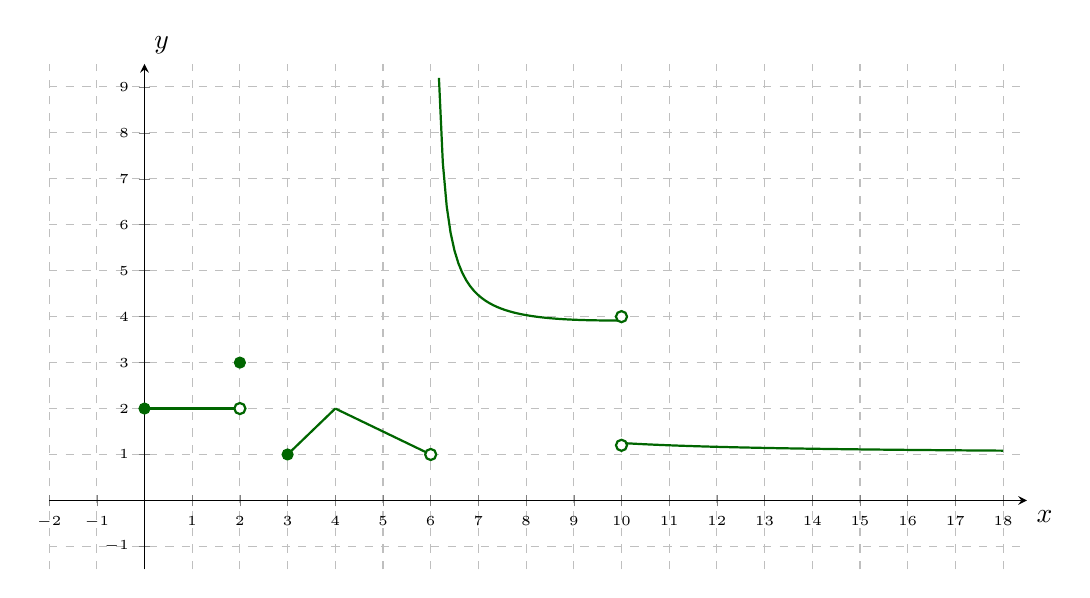
\begin{tikzpicture}
        \begin{axis}[
            axis lines=middle,
            xlabel=$x$,
            ylabel=$y$,
            xmin=-2, xmax=18.5,
            ymin=-1.5, ymax=9.5,
            grid=major,
            grid style={dashed, gray!50},
            xtick={-2,-1,0,1,...,18},
            ytick={-1,0,1,...,9},
            width=14cm,
            height=8cm,
            tick label style={font=\tiny},
            xlabel style={anchor=north west},
            ylabel style={anchor=south west},
            no markers % Tắt các marker tự động
        ]
            % Định nghĩa màu sắc cho đồ thị
            \colorlet{mygreen}{green!40!black}

            % --- Vẽ các đoạn của hàm số ---
            
            % 1. Đoạn ngang y=2, từ x=0 đến x=2
            \addplot[mygreen, thick, domain=0:2] {2};

            % 2. Hình chữ V, từ (3,1) đến (4,2) rồi đến (6,1)
            \addplot[mygreen, thick, domain=3:4] {x-2};
            \addplot[mygreen, thick, domain=4:6] {-0.5*x + 4};

            % 3. Nhánh Hyperbola với tiệm cận đứng x=6
            % Vẽ phần gần tiệm cận, giới hạn chiều cao để không bị vỡ hình
            \addplot[mygreen, thick, domain=6.01:10, samples=50, restrict y to domain=-1.5:10.5] {1/(x-6) + 1/15*x + 3};
            % Vẽ phần còn lại của nhánh hyperbola
            \addplot[mygreen, thick, domain=10:18, samples=50] {1/(x-6) + 1};

            % --- Đánh dấu các điểm đặc biệt ---
            
            % Các điểm được tô đầy (included)
            \addplot[only marks, mark=*, mygreen, mark size=2pt, fill=mygreen] coordinates {
                (0,2)   % Điểm bắt đầu của đoạn ngang
                (2,3)   % Điểm riêng lẻ ở trên
                (3,1)   % Điểm bắt đầu của hình chữ V
            };

            % Các điểm rỗng (excluded)
            \addplot[only marks, mark=o, mygreen, mark size=2pt, draw=mygreen, fill=white, thick] coordinates {
                (2,2)   % Điểm kết thúc của đoạn ngang
                (6,1)   % Điểm kết thúc của hình chữ V
                (10,4)   % Điểm bị loại trừ trên nhánh hyperbola
                (10,1.2) % Điểm bị loại trừ trên nhánh hyperbola
            };

        \end{axis}
    \end{tikzpicture}
    \caption{Hình 3.1.4}
    \label{fig:complex_piecewise_graph}
\end{figure}


\begin{exercise}
Hãy phác họa đồ thị của mỗi hàm số sau đây, và khảo sát tính liên tục hay khả vi của mỗi hàm tại điểm nối.
\begin{enumerate}[label=(\alph*)]
    \item $y = \begin{cases} x^2, & x \le 1, \\ 2x-1, & x > 1. \end{cases}$ \quad (liên tục và khả vi)
    \item $y = \begin{cases} x^2+1, & x \ge 0, \\ x+1, & x < 0. \end{cases}$ \quad (liên tục nhưng không khả vi)
\end{enumerate}
\end{exercise}

\begin{exercise}
Xét $f(x) = \sqrt[3]{x}$. Chứng tỏ rằng $f'(0)$ không tồn tại. Đây là trường hợp tiếp tuyến thẳng đứng. Hãy vẽ đồ thị để minh họa.
\end{exercise}

\begin{exercise}
Xét $f(x) = \sqrt[3]{x^2}$. Chứng tỏ rằng $f'(0)$ không tồn tại. Đây là trường hợp đồ thị có một điểm nhọn (cusp). Hãy vẽ đồ thị để minh họa.
\end{exercise}

\begin{exercise}
Chứng tỏ rằng hàm số $f(x) = |x-6|$ liên tục tại mọi nơi nhưng không khả vi tại $x=6$. Hãy phác họa đồ thị của hàm số này.
\end{exercise}

\begin{exercise}
Cho hàm số $f(x) = \begin{cases} x+1, & x \le 1 \\ 3-x, & 1 < x < 2 \\ \dfrac{1}{x-1}, & x \ge 2. \end{cases}$. Hàm số này khả vi tại những điểm nào? Giải thích.
\end{exercise}